% latex article template

% cheat sheet(eng): http://www.pvv.ntnu.no/~walle/latex/dokumentasjon/latexsheet.pdf
% cheat sheet2(eng): http://www.pvv.ntnu.no/~walle/latex/dokumentasjon/LaTeX-cheat-sheet.pdf
% reference manual(eng): http://ctan.uib.no/info/latex2e-help-texinfo/latex2e.html

% The document class defines the type of document. Presentation, article, letter, etc. 
\documentclass[12pt, a4paper]{article}

% packages to be used. needed to use images and such things. 
\usepackage[pdfborder=0 0 0]{hyperref}
\usepackage[utf8]{inputenc}
\usepackage[english]{babel}
\usepackage{graphicx}
\PassOptionsToPackage{hyphens}{url}

% hides the section numbering. 
\setcounter{secnumdepth}{-1}

% Graphics/image lications and extensions. 
\DeclareGraphicsExtensions{.pdf, .png, .jpg, .jpeg}
\graphicspath{{./images/}}

\title{
	Information systems\\
	project report\\	
}
\author{
	\underline{Group members:} \\
	Bae, Magnus\\
	Bremnes, Jan Alexander Stormark\\
	Krane, Magnus\\
	Sande, Kristian Olafsen\\
	Tørresen, Håvard\\
}
\date{\today}

\hypersetup{
	colorlinks=true,
	linkcolor=black,
	filecolor=red,
	urlcolor=blue
}

\begin{document}
\maketitle
\pagenumbering{arabic}

\newpage
\tableofcontents
\newpage
\section{Introduction}


This report documents the requirement specifications of “NTNUs Ultimate Digital Learning 
platform” (NUDL), which is a proposal for an IT-system for the Norwegian University of 
Science and Technology (NTNU). NUDL proposes to digitalize some of the current processes 
involved in studies at NTNU, such as delivering a complaint on a grade, to ease the 
process for all parties involved and cut an unnecessary load of paperwork. Beyond that 
it also proposes to streamline these processes, along with the processes that are 
already digitalized, under a standardized user interface and an updated security system.

\noindent
The report will begin with an analysis of the current situation, highlighting the 
processes and problems we found most in need of rework and digitalizing. Following, there 
will be an in-depth explanation of how we propose to solve these issues, and how NUDL 
will work and respond when put to use in situations that are managed by other systems 
today.

\section{Background}
In this chapter we will present the background for this project, and review the factors that have
influenced our decisions and vision for this project. 
\section{Old system}
\subsection{Several systems}
Today's system is divided into several semi-independent systems. This is for instance StudentWeb, Eksamensweb, Innsida 2.0, It's Learning, and etc. This means that a student has to go through several systems to do something simple. If you would like to register into a new course, you would have to deal with three different systems (Figure \pageref{fig:Register-old}). If you would like to complain on the grade, you must also interact with 3 systems, some of which demands manual labour from the faculty staff (Figure \pageref{fig:Complain-old}).
\subsection{Complexity}Since the total system is divided into several sub-system, these systems are unnecessary complex and slow. Some of these systems are also:
\begin{itemize}
\item Proprietary closed source.
\item 15 year old code base.
\item Architecturally locked in to Microsoft technologies.
\item Licensing costs.
\end{itemize}This means that they are not easy to upgrade and not very modular. It also means that if we were to upgrade only parts of the current system, it will probably end up just as complex as the current system since we would have to consider the parts that is left. %finn på et bedre navn?
\section{BPMN-models}
	The following BPMN-models\cite{bpmn} describe how we view the current processes of registering to a course, and complaining on a grade, followed by our suggested changes.
All models are from a student's perspective, as that is what we found most interesting.

\subsection{registering to a course}
		
\begin{figure}[H]
    \centering
    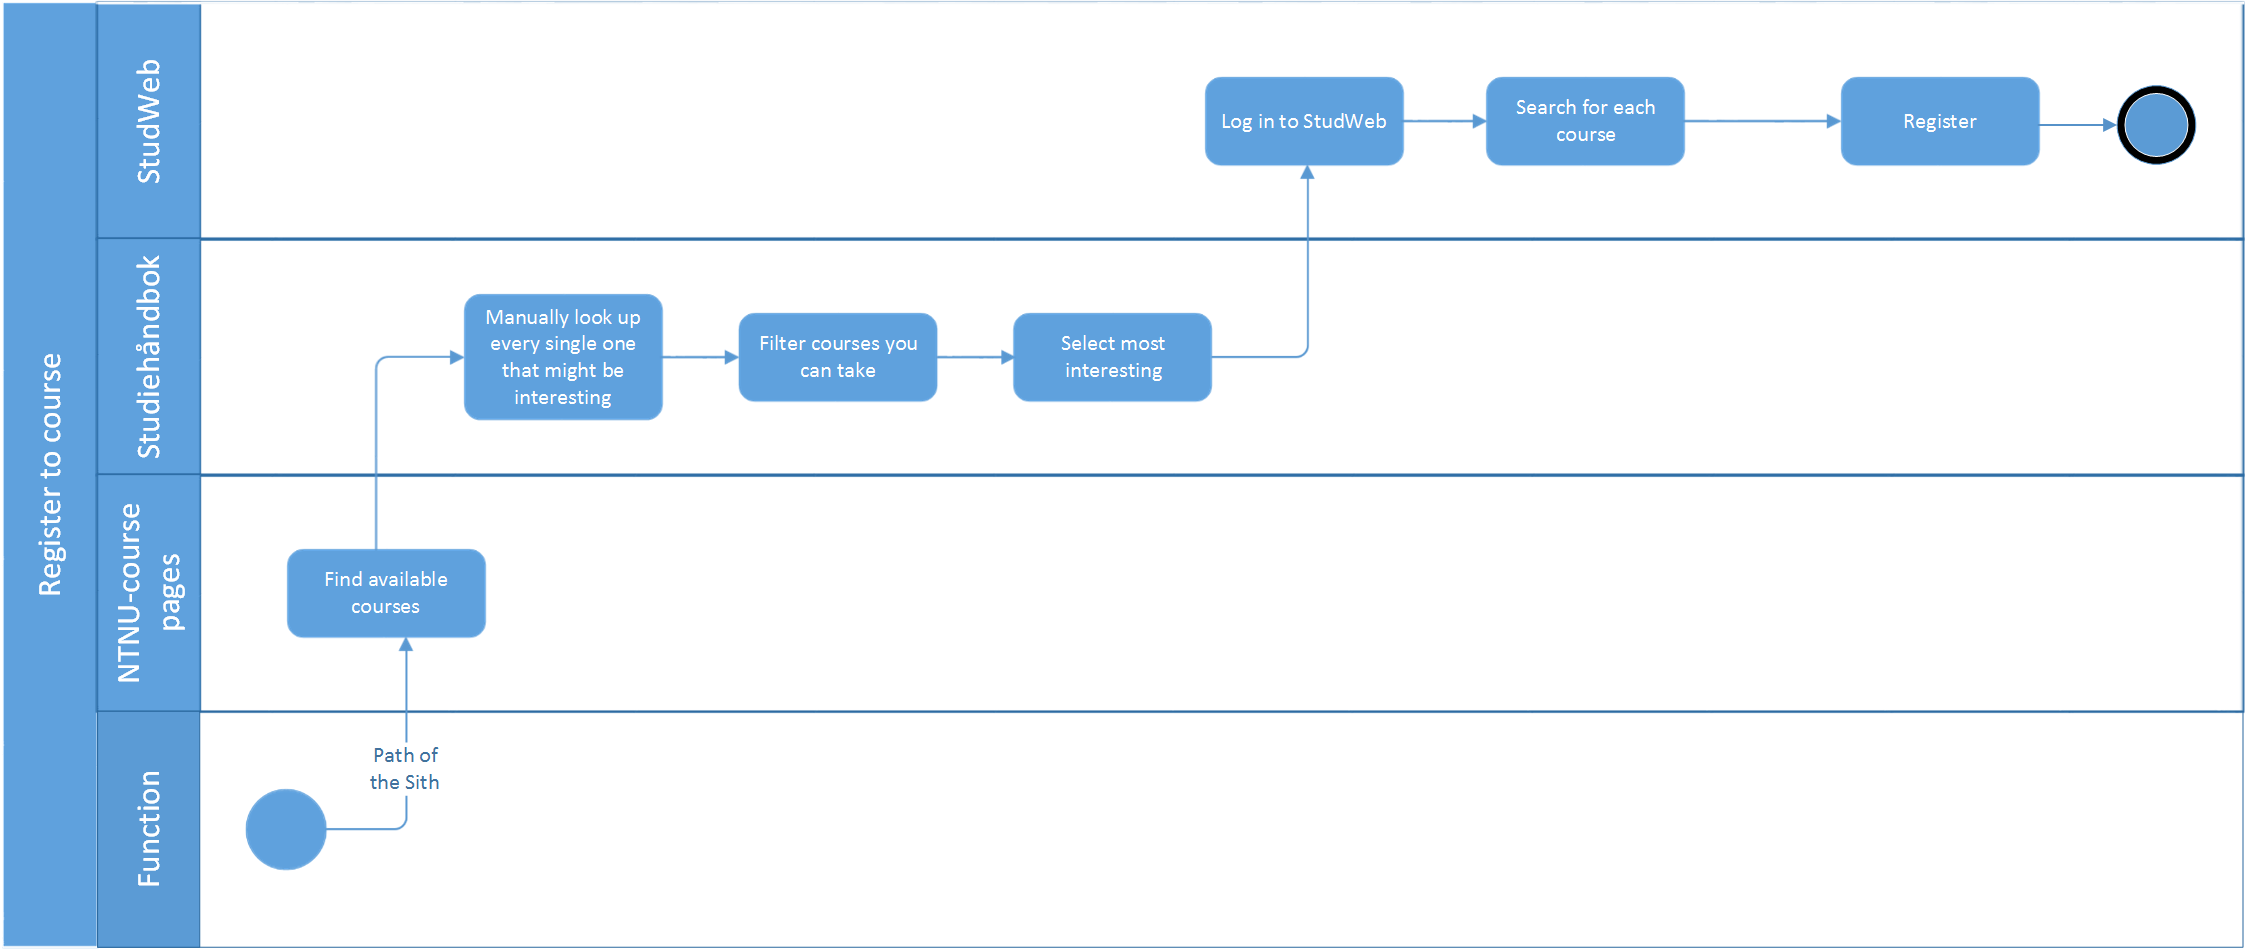
\includegraphics[width=\textheight, angle=-90]{BPMN-register-old}%apparently sets width first and then rotates
    \caption{Our interpretation of the current process of registering to a course.}
    \label{fig:Register-old}
\end{figure}

\begin{figure}[H]
    \centering
    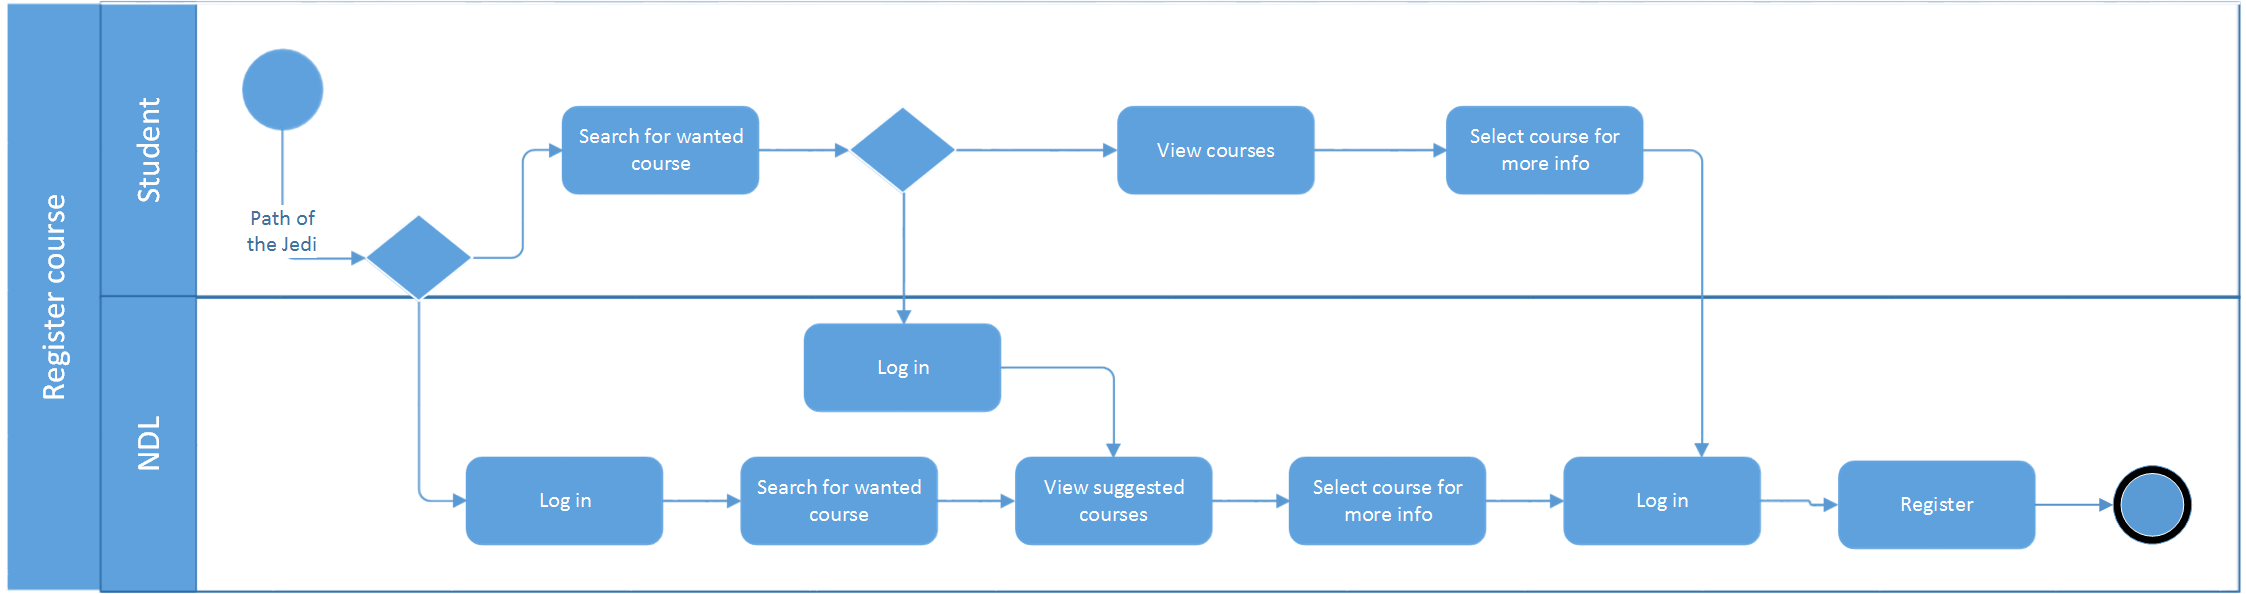
\includegraphics[width=\textheight, angle=-90]{BPMN-register}
    \caption{How we envision our new process of registering to a course to be.}
    \label{fig:Register-new}
\end{figure}

\begin{figure}[H]
    \centering
    \includegraphics[width=\textheight, angle=-90]{BPMN-complain-old}
    \caption{Our interpretation of the current process of complaining on a grade}
    \label{fig:Complain-old}
\end{figure}

\begin{figure}[H]
    \centering
    \includegraphics[width=\textheight, angle=-90]{BPMN-complain}
    \caption{How we envision our new process of complaining to be.}
    \label{fig:Complain-new}
\end{figure}


\cite{bpmn} %fjern senere
\bibliography{bibliography}
\bibliographystyle{acm}

\end{document}
